\chapter{تکمیل شبکه‌های تعاملات پروتئینی با استفاده از گرافلت کرنل گاوسی}\label{chap:network-completion-problem-ppi}
همانطور که در فصل \ارجا{chap:protein_function_prediction} به آن اشاره شد، پروتئین‌ها اساس فعالیت‌های سلولی را تشکیل می‌دهند. اما پروتئینی که بتواند به تنهایی مفید باشد نادر است. آن‌ها معمولاً با اتصال به یکدیگر و تشکیل یک ساختار مرکب است که می‌توانند فعالیت‌های خود را انجام ‌دهند. به عنوان مثال، در فرآیند رونویسی از DNA\پانوشت{\متنلاتین{DNA replication}}، ماشین \متنلاتین{replisome} حداقل از تعامل فیزیکی ۴۰ پروتئین برای انجام وظیفه خود استفاده می‌کند\جستار{Macneill_2012}. مطالعه این تعاملات، نقش مهمی در درک سامانه‌های زیستی خواهد داشت و کشف دلایل و درمان بسیاری از بیماری‌ها به این وسیله ممکن خواهد بود\جستار{Ryan_2005}.

به دلیل اهمیت فراوان موضوع، چندین روش آزمایشگاهی برای یافتن این تعاملات ابداع شده‌اند. پایگاه داده \متنلاتین{IntAct}\جستار{Hermjakob_2004} حدود ۱۷۰ روش آزمایشگاهی را در وب‌سایت خود لیست کرده‌است که می‌توانند برای این منظور استفاده شوند. بعضی از این روش‌ها \خمیده{کم‌توان}\پانوشت{\متنلاتین{low-throughput}} هستند، یعنی در هر بار آزمایش تنها می‌توانند تعداد اندکی از تعاملات را شناسایی کنند. از این تکنیک‌ها بیشتر برای راستی سنجی پیش‌بینی‌ها استفاده می‌شود و قابلیت استفاده گسترده برای تشخیص تمام تعاملات را ندارند. اما بعضی دیگر در اصطلاح \خمیده{پر‌توان}\پانوشت{\متنلاتین{high-throughput}} هستند و در هر بار آزمایش، تعاملات بین چندین پروتئین را تشخیص می‌دهند. در دسته‌بندی دیگر، می‌توان این روش‌ها را در دو گروه تشخیص روابط دوتایی و چندتایی جای داد، به این معنی که بعضی روش‌ها تعامل مستقیم دو پروتئین را رصد می‌کنند در حالی که بعضی دیگر تعامل بین دو یا چند پروتئین را تشخیص می‌دهند که ممکن است مستقیم و یا غیر مستقیم در ارتباط باشند.

مشکل مشترک روش‌های آزمایشگاهی، درصد خطای بالاست. مثلاً برای تکنیک \متنلاتین{Y2H}\پانوشت{\متنلاتین{Yeast two-hybrid}}، خطا تا حدود ۷۰ درصد تخمین زده شده‌است\جستار{Deane_2002}. از آنجایی که داده‌های موجود اکثراً نتیجه‌ی روش‌های پرتوان هستند، خطای بالایی دارند. چه اینکه ممکن است تعاملاتی را که وجود ندارد، تشخیص دهند و چه تعاملاتی که وجود دارند را شناسایی نکنند.

راه حل‌های بیوانفورماتیکی متعددی برای غربالگری داده‌های موجود و پیش‌بینی تعاملات، ارائه شده‌است. که در ادامه مروری بر آن‌ها خواهیم داشت.

\section{روش‌های محاسباتی پیش‌بینی تعاملات پروتئینی}
این روش‌ها را می‌توان به چهار دسته تقسیم کرد: روش‌های مبتنی بر اطلاعات ژنی، ساختار پروتئین‌ها، یادگیری ماشین و ساختار شبکه‌های تعاملات پروتئینی.

\subsection{روش‌های مبتنی بر اطلاعات ژنی}
\subsubsection{همسایگی ژن‌ها}
همسایگی ژن\پانوشت{\متنلاتین{gene neighbouring}} یا هم‌محلی ژن‌ها\پانوشت{\متنلاتین{gene co-localization}} یکی از اولین و ساده‌ترین روش‌های محاسباتی برای پیش‌بینی تعاملات پروتئینی است\جستار{Dandekar_1998}\جستار{Tamames_1997}. ایده اصلی، این مشاهده است که در ژنوم، ژن‌های مرتبط کنار هم قرار می‌گیرند. مهمترین مشکل این روش، این است که برخلاف پروکاریوت‌ها، برای موجودات یوکاریوتی چنین فرضی صحیح نیست. پس همسایگی ژنی نمی‌تواند بسیاری از تعاملات بین پروتئین‌هایی که ژن‌هایشان کنار هم قرار نگرفته‌اند را شناسایی کند. مشکل دیگر این است که نتایج حاصل از این روش، وابستگی مستقیمی به ژنوم تحت بررسی دارد و قابل بسط به دیگر موجودات نیست\جستار{Muley_2012}.

\subsubsection{ارتباط فیلوژنی}
در اینجا، تعاملات پروتئینی بر اساس شباهت \خمیده{پروفایل فیلوژنی}\پانوشت{\متنلاتین{phylogenic profile}} پیش‌بینی می‌شود\جستار{Guimaraes_2006}\جستار{Juan_2008}. پروفایل فیلوژنی برای یک پروتئین، برداری شامل درایه‌های یک و صفر است که وجود یا عدم وجود آن پروتئین در مجموعه‌ای از ارگانسیم‌ها را مشخص می‌کند. ایده اصلی این است که دو ژنِ مرتبط از لحاظ عملکرد، در بین گونه‌هایی که به لحاظ تکاملی از هم دور هستند، یا با هم حضور دارند یا هیچ‌کدام حضور ندارند. چون ژنی که به تنهایی کارایی ندارد در روند تکامل حذف خواهد شد. ارتباط فیلوژنی، مشکل اول روش همسایگی ژنی را حل کرده‌است و می‌تواند ارتباط ژن‌های با فاصله روی ژنوم را هم تشخیص دهد. اما بازهم نتایج به تعداد و توزیع ژنوم مورد استفاده، وابسته است. مشکل دیگر این روش آن است که بسیاری از پروتئین‌های حیاتی در همه یا اکثر موجودات وجود دارند و ارتباط فیلوژنی نمی‌تواند تعامل بین آن‌ها را تشخیص دهد\جستار{Muley_2012}.

\subsubsection{ادغام ژن‌ها}
مشاهدات نشان داده است که ژن‌های مرتبط می‌توانند در قالب یک ژن چند منظوره ادغام شوند، چیزی که نتیجه آن در اصطلاح یک پروتئین \متنلاتین{Rosetta Stone} است. روش ادغام ژن\پانوشت{\متنلاتین{Gene Fusion}} از اطلاعات تکاملی و مقایسه ژنوم بهره می‌برد\جستار{Marcotte_1999}\جستار{Enright_1999} و به نوعی بهبود یافته دو روش قبلی است. بهترین ویژگی این روش استفاده از مفهومی است که اطلاعات بسیاری راجع به پروتئین‌های مرتبط بدست می‌دهد. اما مشکل اینجاست که در طبیعت ادغام ژن‌ها به خصوص در پروکاریوت‌ها زیاد اتفاق نمی‌افتد.

\subsection{روش‌های مبتنی بر ساختار پروتئین}
\subsubsection{ساختار اول}
از ساختار اول پروتئین یا توالی اسید‌های آمینه به همراه اطلاعات قبلی از تعاملات پروتئین می‌توان اطلاعاتی استخراج کرد که در پیش‌بینی تعاملات جدید مورد استفاده قرار می‌گیرد\جستار{Matthews_2001}\جستار{Bock_2001}. در این روش، چند جفت پروتئین که با هم تعامل دارند انتخاب شده و تکه‌های توالی که در بین آن‌ها مشترک است به عنوان نشانه در نظر گرفته می‌شوند. این نشانه‌ها بر روی توالی‌ مربوط به دیگر پروتئین‌ها جستجو شده و وجود آن‌ها احتمالاً به معنی تعامل این پروتئین‌هاست.

\subsubsection{ساختار سوم}
استفاده از ساختار سوم پروتئین‌ها برای پیش‌بینی تعاملات\جستار{Aloy_2003}\جستار{Hue_2010} بسیار منطقی است زیرا به هر حال پروتئین‌ها از طریق مقر‌های اتصال که توسط ساختار سوم آن‌ها تعیین می‌شود با هم ارتباط برقرار می‌کنند. مهمترین محدودیت این روش کمبود پروتئین‌هایی است که ساختار سه‌بعدیشان استخراج شده‌است. در مقایسه با روش‌های دیگر، نتایج این روش اطلاعات دقیق‌تری از نحوه تعامل و اتصال پروتئین‌ها بدست می‌دهند، از جمله اینکه مقر اتصال کجاست و ویژگی‌های بیوفیزیکی آن چیست.

\subsection{روش‌های مبتنی بر یادگیری ماشین}
تمام روش‌هایی که در بالا به آن‌ها اشاره شد بر مبنای اصول اولیه زیستی پایه‌ریزی شده‌اند. اما دسته دیگری از روش‌ها وجود دارند که بر مبنای یادگیری عمل می‌کنند\جستار{Najafabadi_2008}\جستار{HsinLiu_2012}. به این صورت که از پروتئین‌ها یا هر دو پروتئین به صورت جفت، برداری از ویژگی‌ها استخراج می‌شود. این بردارها به عنوان ورودی یک ماشین دسته‌بندی مثل \متنلاتین{SVM} مورد استفاده قرار می‌گیرد تا ماشین بتواند بین پروتئین‌هایی که در تعامل هستند و آن‌هایی که قادر به تعامل نیستند تمایز قائل شود. در این روش‌ از داده‌هایی مثل بیان ژن‌، اطلاعات مربوط به توالی و ساختار پروتئین‌ برای ساخت بردارهای ویژگی استفاده می‌شود. اما برخلاف روش‌های قبل، در اینجا اصول و فرضیات زیستی در نحوه کار ماشین دخیل نیستند. در واقع ماشین به صورت یک جعبه سیاه عمل می‌کند و ما فقط شاهد نتایج هستیم.

\subsection{روش‌های مبتنی بر ساختار شبکه}
در نگاه ریاضیاتی به مسئله، شبکه تعاملات پروتئین، گرافی است که در آن مجموعه
پروتئین‌های یک ارگانیسم، رئوس گراف و تعاملات بین آن‌ها، یال‌های این گراف را تشکیل می‌دهند. یعنی بین دو رأس، یال قرار می‌دهیم اگر پروتئین‌های متناظر تعامل داشته باشند. به اختصار به این شبکه‌، \متنلاتین{PIN}\پانوشت{\متنلاتین{Protein Interaction Network}} گفته می‌شود.

این شبکه‌ها توپولوژی یا ساختاری دارند که آن‌ها را از گراف‌های کاملاً تصادفی متمایز می‌کند. از این ویژگی‌های ساختاری برای تشخیص تعاملات اشتباه و پیش‌بینی تعاملات جدید و یا رتبه بندی تعاملات موجود استفاده می‌شود\جستار{Saito_2003}\جستار{Chen_2006}. اما به دلیل نرخ بالای خطا در شبکه‌های موجود، تشخیص ساختار و مدل‌سازی آن، مسئله ساده‌ای نیست و هنوز توافقی روی مدل مناسب برای \متنلاتین{PIN}ها صورت نگرفته است\جستار{Han_2005}.

\section{روش پیشنهادی}
همانطور که در فصل \ارجا{chap:protein_function_prediction} به آن اشاره شد، معمولاً پروتئین‌هایی که شکل یکسان دارند، عملکردشان نیز یکسان است. و باز در ابتدای همین فصل، اشاره شد که پروتئین‌ها با اتصال به دیگر پروتئین‌هاست که می‌توانند نقش خود را انجام دهند. بنابراین منطقی است که نتیجه بگیریم: پروتئین‌های مشابه از لحاظ ساختاری، احتملاً تعاملات مشابه‌ای هم دارند. پس اگر دو پروتئین «آ» و «ب» با هم تعامل داشته باشند و پروتئین «پ» شبیه «آ» و پروتئین «ت» شبیه «ب» باشد، می‌توانیم نتیجه بگیریم «پ» و «ت» هم تعامل دارند. عکس این موضوع نیز صادق است. یعنی اگر دو پروتئین «آ» و «ب» تعامل نداشته باشند، می‌توانیم نتیجه بگیریم که احتمالاً «پ» و «ت» هم تعامل ندارند. هرچند همه چیز تا این حد ساده نیست و قوانین پیچیده‌تری بر تعاملات حکم فرماست، اما این ساده‌سازی باعث می‌شود به اطلاعات کمتری از پروتئین برای پیش‌بینی تعاملات آن، نیاز داشته باشیم.

بر همین مبنا، روش پیشنهادی در این پایان‌نامه استفاده از گرافلت‌کرنل گاوسی به همراه ماشین \متنلاتین{SVM} روی ساختار سوم پروتئین‌هاست. می‌خواهیم ماشین \متنلاتین{SVM} را طوری آموزش دهیم که یک ورودی به صورت دوتایی $(p_i,p_j)$ (که $p_i$ و $p_j$ پروتئین هستند) دریافت کند و بگوید این دو پروتئین تعامل دارند یا خیر. برای آموزش این ماشین نیاز به مجموعه‌ای به صورت
\begin{equation*}
(x_1,y_1),...,(x_N,y_N) \in \mX \times \mY
\end{equation*}
داریم که در آن $\mX \subseteq P\times P$ مجموعه دوتایی‌های $(p_i,p_j)$ است که $p_i,p_j \in P$ پروتئین هستند و  $\mY = \left\lbrace-1,+1 \right\rbrace$ برچسب هر دوتایی از $\mX$ است. برچسب $+1$ نشان‌دهنده تعامل بین دو پروتئین و برچسب $-1$ نشان‌دهنده عدم وجود تعامل بین آن دو است. با در اختیار داشتن این مجموعه، تابع کرنل $k: \mX\times \mX \mapsto \R$ را به صورت زیر تعریف می‌کنیم:
\begin{equation*}
k((p_i,p_j),(p_u,p_v)) = k_{GGK}(p_i,p_u) + k_{GGK}(p_j,p_v)
\end{equation*}
که در آن، $k_{GGK}$ تابع گرافلت کرنل گاوسی است. $k$ یک کرنل مثبت معین است زیرا از جمع دو کرنل مثبت معین حاصل شده‌است (بخش \ارجا{sec:positive-semidefinite-kernels} را ببینید).

\section{داده‌ها}
دقت یک ماشین دسته‌بندی مثل \متنلاتین{SVM}، وابستگی زیادی به دقت داده‌های اولیه دارد. در مورد دقت داده‌های مربوط به تعاملات پروتئینی، با دو مشکل روبرو هستیم. مشکل اول در ارتباط با داده‌هایی است که بیان می‌کنند دو پروتئین در تعامل هستند. همانطور که گفته شد خطای این داده‌ها بخصوص برای آن‌هایی که از روش‌های پرتوان بدست آمده‌اند، بالاست. مشکل دوم، عدم وجود اطلاعات کافی در مورد تعاملاتی است که مطمئن هستیم وجود ندارند. یعنی اگر بین دو پروتئین، تعاملی گزارش نشده باشد، نمی‌توان نتیجه گرفت که این دو حتماً تعامل ندارند.

برای رفع مشکل اول، باید داده‌های چند پایگاه را پالایش کرده و تعاملاتی را انتخاب کنیم که حداقل در دو یا سه آزمایش مجزا، گزارش شده‌باشند. خوشبختانه، پایگاه‌هایی وجود دارند که این تعاملات را استخراج کرده و آن‌ها را به عنوان داده‌های با اطمینان بالا در اختیار قرار می‌دهند.

اما برای رفع مشکل دوم، پایگاهی با نام \متنلاتین{Negatome}\جستار{Smialowski_2010} وجود دارد که به طور دقیق عدم تعامل جفت پروتئین‌ها را گزارش می‌دهد. با این وجود، داده‌های این پایگاه کافی نیست و اشتراک بین پروتئین‌های این پایگاه با پروتئین‌هایی که برای رفع مشکل اول انتخاب می‌کنیم (برای تشکیل مجموعه $P$) بسیار کم است بطوری که در فرآیند استخراج داده برای آزمون روش پیشنهادی در این فصل، نسبت داده‌های مثبت (برچسب $+1$) به داده‌های منفی (برچسب $-1$) استخراج شده از Negatome ، سیزده به یک بود. روش دیگری که معمولاً برای حل این مشکل استفاده می‌شود، ایجاد دوتایی هایی است که هر پروتئین آن، متعلق به واحد سلولی مجزایی است\جستار{Veres_2014}. منظور از واحد سلولی\پانوشت{\متنلاتین{Cellular compartment}}، قسمت‌هایی از سلول است که توسط یک غشاء از باقی مواد سلول جدا شده باشند. به طور کلی چهار نوع واحد سلولی داریم که عبارت‌اند از هسته، قسمت داخلی شبکه آندوپلاسمی\پانوشت{\متنلاتین{Intercisternal space}}، سیتوپلاسم، و اندامک‌های دیگر مثل میتوکندری\پانوشت{\متنلاتین{Mitochondrion}} و واکول\پانوشت{\متنلاتین{Vacuole}} و \ldots . از آن‌جایی که این قسمت‌ها با غشاء از دیگر مواد جدا شده‌اند، پس پروتئین‌های موجود در آن‌ها به ندرت قادر به تعامل با دیگر پروتئین‌های محلول در سلول هستند. پایگاه \متنلاتین{ComPPI}\جستار{Veres_2014} این داده‌ها را فراهم می‌آورد.

برای جمع آوری داده‌های مثبت، از پایگاه‌های \متنلاتین{DIP}، \متنلاتین{IntAct} و \متنلاتین{BioGrid} استفاده کرده و 20454 تعامل بین 6811 پروتئین گونه انسانی را در قالب شماره دسترسی \متنلاتین{UniProt} از بین تعاملاتی که حداقل دوبار در مقالات دیده شده بودند، استخراج نمودیم. از بین این تعاملات، آن‌هایی که حداقل یکی از پروتئین‌هایشان بدون ساختار سوم مشخص بودند، حذف شدند. در نتیجه، تعداد 9403 تعامل بین 2697 پروتئین با ساختار سوم مشخص باقی ماند. برای هر شماره دسترسی \متنلاتین{Uniprot}، ممکن است بیش از یک ساختار سوم با شناسه \متنلاتین{PDB} مشخص شده باشد. در این صورت ما ساختار سومی را که بیشترین دقت (کمترین \متنلاتین{resolution}) را داشت، انتخاب کرده و در قالب فایل \متنلاتین{PDB} از پایگاه \متنلاتین{RCSB} دریافت کردیم.

برای تشکیل مجموعه داده‌های منفی، دوتایی‌های موجود در پایگاه \متنلاتین{Negatome} بین ۲۶۹۷ پروتئین انتخاب شده در مرحله قبل را بازیابی کردیم. از این راه، ۶۸۷ دوتایی بدست آمد. برای ایجاد تعادل بین تعداد داده‌های مثبت و منفی، 10716 دوتایی دیگر بین پروتئین‌های انتخاب شده که در واحد سلولی متفاوتی بودند از پایگاه \متنلاتین{ComPPI} استخراج شد که تعداد داده‌های منفی را جمعاً به ۱۱۴۰۳ دوتایی رساند.

در مجموع، ۲۰۸۰۶ دوتایی بین ۲۶۹۷ پروتئین برای سنجش میزان دقت روش پیشنهادی گردآوری شد. هر پروتئین، به صورت گراف با در نظر گرفتن موقعیت اتم کربن آلفا و فاصله ۶ آنگسترم مطابق بخش \ارجا{sec:protein-to-graph} مدل سازی گردید.

\section{شرایط آزمون}
مشابه فصل قبل، برای آزمون روش پیشنهادی از زبان برنامه نویسی \متنلاتین{C++} جهت پیاده‌سازی کرنل‌ و از زبان \متنلاتین{R} به منظور یادگیری روی ماشین \متنلاتین{C-SVM} و تحلیل داده‌ها استفاده کردیم. آزمون در قالب \متنلاتین{10-fold cross validation}، ده بار تکرار شد.

\section{مقایسه و بررسی نتایج}
در این بخش به مقایسه روش پیشنهادی که به اختصار GKPIP می‌نامیم با روش \متنلاتین{FpClass}\جستار{Kotlyar_2014} می‌پردازیم. \متنلاتین{FpClass} روشی مبتنی بر داده‌کاوی است که اطلاعات مختلفی از پروتئین‌ها را برای پیش‌بینی تعامل، مورد استفاده قرار می‌دهد. این اطلاعات شامل دامین‌ها، تغییرات بعد از ترجمه\پانوشت{post-translational modifications}، برچسب‌های \متنلاتین{GO}، توپولوژی شبکه تعاملات، هم‌بیانی ژن‌ها و ویژگی‌های فیزیکی و شیمیایی پروتئین‌هاست. در این روش، بطور مجزا برای هر ويژگی، یک احتمال به هر تعامل نسبت داده می‌شود. این عدد نشان می‌دهد که بر مبنای آن ویژگی خاص، چقدر وجود هر تعامل محتمل است. در نهایت با استفاده از شبکه بیزی، این احتمالات ترکیب شده و برای هر تعامل یک احتمال نهایی بدست می‌آید.  شبکه بیزی بکار رفته در این روش، روی داده‌های بسیار بزرگ شامل 2 میلیون تعامل آموزش داده شده و  نتایج بسیار خوبی داشته است.

به دو دلیل ما نمی‌توانیم ماشین \متنلاتین{SVM} طراحی شده را روی این حجم از داده آموزش دهیم. دلیل اول، عدم وجود امکانات فنی است. آموزش این ماشین روی مجموعه بیست هزارتاییِ تشکیل شده، نیاز به حداقل ۱۶ گیگابایت حافظه دارد. برای مجموعه دو میلیونی باید حافظه‌ی بسیار بسیار بیشتری در اختیار داشت. مشکل دوم، عدم تعادل بین مجموعه مثبت و منفی است بطوری که  تقریباً ۹۷٪ از تعاملات این مجموعه دو میلیونی، در مجموعه منفی قرار می‌گیرند. برای ماشین \متنلاتین{SVM} این عدم تعادل به معنی تشخیص تمام تعاملات با برچسب منفی است. بنابراین برای مقایسه، ما \متنلاتین{FpClass} را روی داده‌های معرفی شده در بخش قبل، آموزش دادیم.

شکل \ارجا{fig:roc-curve} نمودار \متنلاتین{ROC} برای دو روش \متنلاتین{GKPIP} و \متنلاتین{FpClass} را نشان می‌دهد. سطح زیر منحنی (\متنلاتین{AUROC}) برای \متنلاتین{GKPIP} برابر ۰.۸۵ و برای \متنلاتین{FpClass} برابر ۰.۵ است. به نظر می‌رسد عدم توانایی \متنلاتین{FpClass} در یادگیری روی این مجموعه، به دلیل حجم کم داده‌هاست. 

\begin{figure}[ht]
\center{
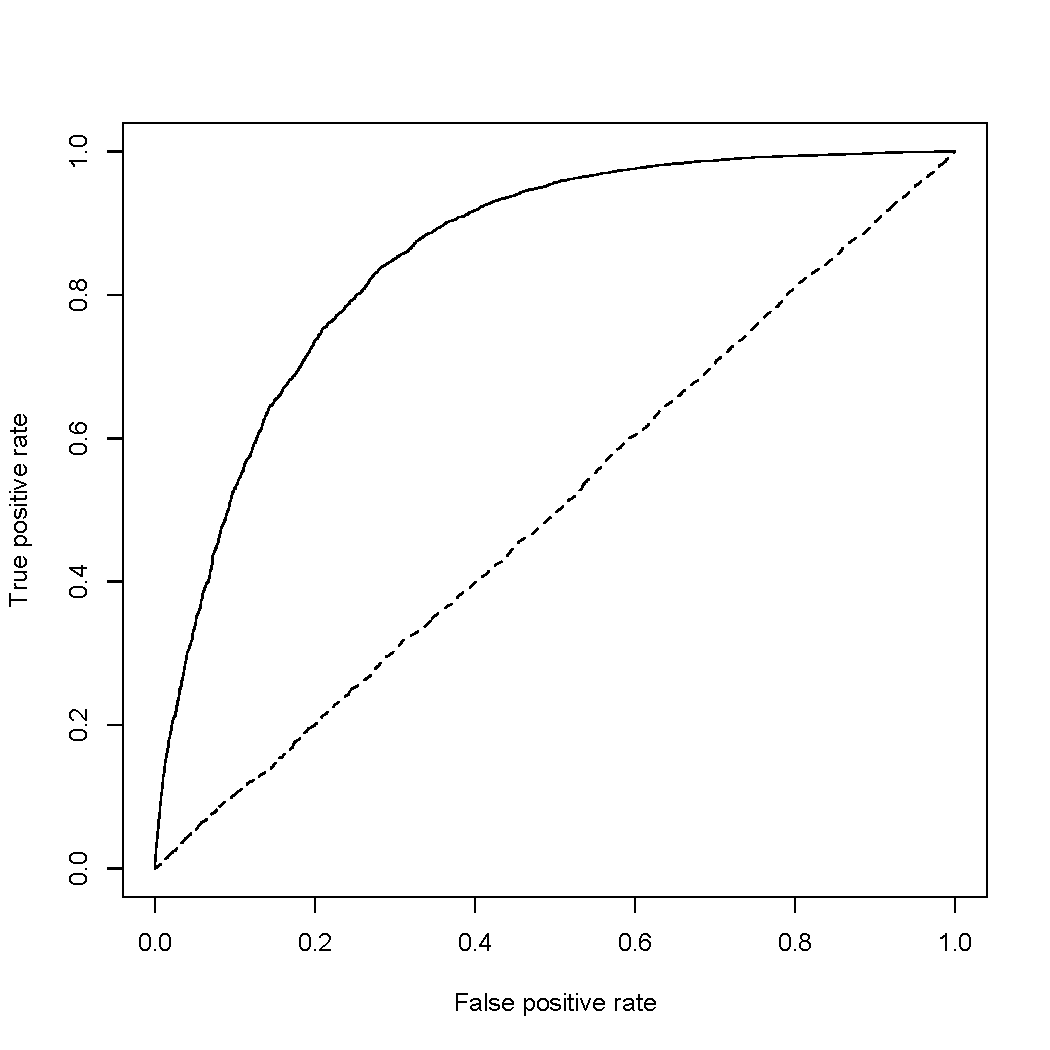
\includegraphics[scale=0.5]{./roc.pdf}
}
\caption{
منحنی \متنلاتین
‫{‬ROC‫}‬
برای 
\متنلاتین{
GKPIP
} (خط صاف) و \متنلاتین{
FpClass
‫}‬
‫(‬خط نقطه‌چین).
}
\label{fig:roc-curve}
\end{figure}

همانطور که گفته شد، در روش \متنلاتین{GKPIP}، تنها از ساختار سوم پروتئین‌ها برای یادگیری و پیش‌بینی تعاملات استفاده می‌شود. استفاده از ساختار سوم، می‌تواند یک نقطه ضعف باشد. پروتئین‌هایی که ساختار سوم معلوم دارند، در مقایسه با پروتئین‌هایی که توالی مشخص دارند، بسیار کم‌اند و همین امر باعث ایجاد محدودیت در یادگیری و همچنین محدودیت در استفاده از این روش می‌شود. در مقابل، استفاده از انواع ویژگی‌ها، همانطور که در \متنلاتین{FpClass} مشاهده می‌کنیم، نیز یک نقطه ضعف است. زیرا برای بسیاری از پروتئین‌ها، اطلاعاتی نظیر دامین‌ها، تغییرات بعد از ترجمه، برچسب‌های \متنلاتین{GO} و \ldots مشخص نیستند و یا درجه اطمینان پایینی دارند.

\section{جمع‌بندی}
در این فصل به بررسی مسئله‌ی تکمیل شبکه‌های تعاملات پروتئینی پرداختیم. با استفاده از گرافلت کرنل گاوسی، روشی برای پیش‌بینی تعاملات ارائه دادیم که با توجه به آزمون انجام شده، در مقایسه با یکی از بهترین روش‌های موجود در این زمینه یعنی \متنلاتین{FpClass} عملکرد بهتری دارد. همانطور که گفته شد، یکی از مهمترین ضعف‌های این روش وابستگی به ساختار سوم پروتئین‌هاست. مطالعات بعدی، می‌تواند با استفاده از مفهوم \متنلاتین{template} برای توالی‌ها، این ضعف را پوشش دهد. یعنی برای هر توالی، با توجه به پروتئین‌های مشابه (که ساختار سوم مشخص دارند)، یک ساختار سوم در نظر گرفته شود. البته بهبود‌های دیگری هم می‌توان برای این روش در نظر گرفت. به عنوان مثال ساخت گراف از روی پروتئین، می‌تواند محدود به اسید‌های آمینه‌ای باشد که سطح در دسترس\پانوشت{\متنلاتین{RSA}} بالاتری دارند. زیرا این قسمت‌ها هستند که در تعاملات نقش بازی می‌کنند و می‌توان با ساخت گراف روی آن‌ها، قسمت‌های بی اهمیت پروتئین را حذف نمود. 
